% Author: Raoul Kessels
\documentclass[12pt]{standalone}
\usepackage{tikz}
\usetikzlibrary{positioning}
% The face style, can be changed
\tikzset{face/.style={shape=circle,minimum size=4ex,shading=radial,outer sep=0pt,
        inner color=white!50!yellow,outer color= yellow!70!orange}}
%% Some commands to make the code easier
\newcommand{\emoticon}[1][]{%
  \node[face,#1] (emoticon) {};
  %% The eyes are fixed.
  \draw[fill=white] (-1ex,0ex) ..controls (-0.5ex,0.2ex)and(0.5ex,0.2ex)..
        (1ex,0.0ex) ..controls ( 1.5ex,1.5ex)and( 0.2ex,1.7ex)..
        (0ex,0.4ex) ..controls (-0.2ex,1.7ex)and(-1.5ex,1.5ex)..
        (-1ex,0ex)--cycle;}
\newcommand{\pupils}{
  %% standard pupils
  \fill[shift={(0.5ex,0.5ex)},rotate=80] 
       (0,0) ellipse (0.3ex and 0.15ex);
  \fill[shift={(-0.5ex,0.5ex)},rotate=100] 
       (0,0) ellipse (0.3ex and 0.15ex);}

\newcommand{\emoticonname}[1]{
  \node[below=1ex of emoticon,font=\footnotesize,
        minimum width=4cm]{#1};}
\begin{document}
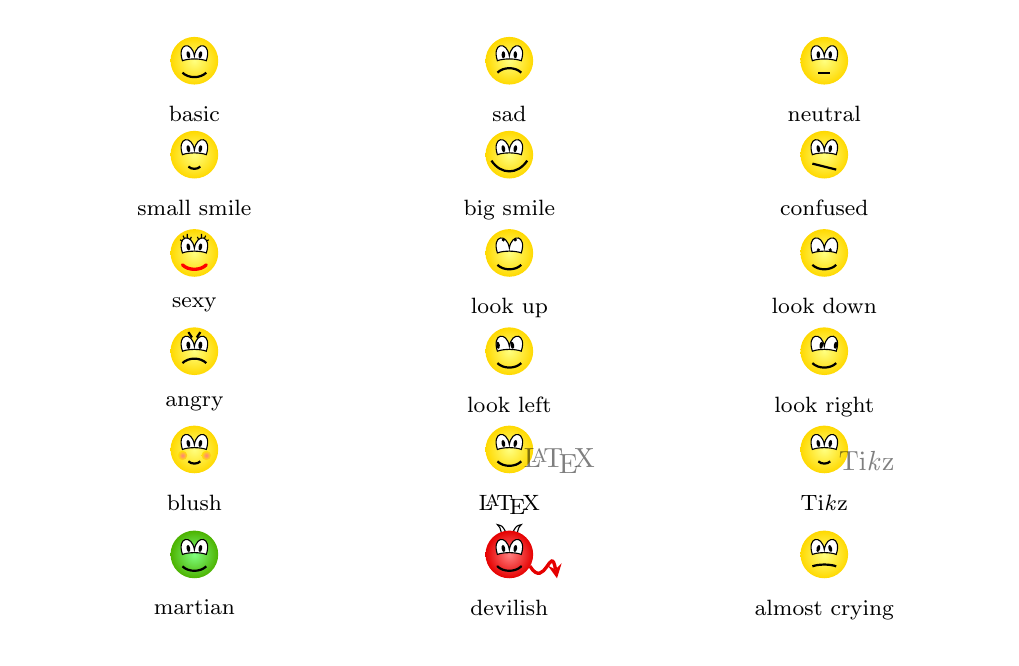
\begin{tikzpicture}
  \matrix {
    \emoticon\pupils\emoticonname{basic}
    %% mouth
    \draw[thick] (-1ex,-1ex)
                 ..controls (-0.5ex,-1.5ex)and(0.5ex,-1.5ex)..(1ex,-1ex);
  &
    \emoticon\emoticonname{sad}
    %% pupils
    \fill[shift={( 0.5ex,0.5ex)},rotate=90] (0,0) ellipse (0.3ex and 0.15ex);
    \fill[shift={(-0.5ex,0.5ex)},rotate=90] (0,0) ellipse (0.3ex and 0.15ex);
    %% mouth
    \draw[thick] (-1ex,-1ex)..controls
        (-0.5ex,-0.5ex)and(0.5ex,-0.5ex)..(1ex,-1ex);
  &
    \emoticon\emoticonname{neutral}
    %% pupils
    \fill[shift={( 0.5ex,0.5ex)},rotate=90] (0,0) ellipse (0.3ex and 0.15ex);
    \fill[shift={(-0.5ex,0.5ex)},rotate=90] (0,0) ellipse (0.3ex and 0.15ex);
    %% mouth
    \draw[thick] (-0.5ex,-1ex)--(0.5ex,-1ex);
  \\
    \emoticon\pupils\emoticonname{small smile}
    %% mouth
    \draw[thick] (-0.5ex,-1ex)
                 ..controls (-0.25ex,-1.25ex)and(0.25ex,-1.25ex)..(0.5ex,-1ex);
  &
    \emoticon\pupils\emoticonname{big smile}
    %% mouth
    \draw[thick] (-1.5ex,-0.5ex)
               ..controls (-0.7ex,-1.7ex)and(0.7ex,-1.7ex)..(1.5ex,-0.5ex);
  & 
    \emoticon\pupils\emoticonname{confused}
    %% mouth
    \draw[thick] (-1ex,-0.75ex)--(1ex,-1.25ex);
  \\
    \emoticon\pupils\emoticonname{sexy}
    %% mouth
    \draw[very thick,red,line cap=round] (-1ex,-1ex)
               ..controls (-0.5ex,-1.5ex)and(0.5ex,-1.5ex)..(1ex,-1ex);
    %% eyelashes
    \draw (0.60ex,1.20ex)--(0.60ex,1.60ex)
          (0.85ex,1.25ex)--(0.95ex,1.45ex)
          (1.00ex,1.00ex)--(1.20ex,1.10ex)
          (0.35ex,1.15ex)--(0.25ex,1.35ex)
          (-0.60ex,1.20ex)--(-0.60ex,1.60ex)
          (-0.85ex,1.25ex)--(-0.95ex,1.45ex)
          (-1.00ex,1.00ex)--(-1.20ex,1.10ex)
          (-0.35ex,1.15ex)--(-0.25ex,1.35ex);
  & 
    \emoticon\emoticonname{look up}
    %% pupils
    \fill[shift={( 0.5ex,1.1ex)},rotate= 80] (0,0) ellipse (0.15ex and 0.15ex);
    \fill[shift={(-0.5ex,1.1ex)},rotate=100] (0,0) ellipse (0.15ex and 0.15ex);
    %% mouth
    \draw[thick] (-1ex,-1ex)..controls
        (-0.5ex,-1.5ex)and(0.5ex,-1.5ex)..(1ex,-1ex);
  & 
    \emoticon\emoticonname{look down}
    %% pupils
    \fill[shift={( 0.5ex,0.25ex)},rotate= 80] (0,0) ellipse (0.15ex and 0.15ex);
    \fill[shift={(-0.5ex,0.25ex)},rotate=100] (0,0) ellipse (0.15ex and 0.15ex);
    %% mouth
    \draw[thick] (-1ex,-1ex)..controls
        (-0.5ex,-1.5ex)and(0.5ex,-1.5ex)..(1ex,-1ex);
  \\
    \emoticon\pupils\emoticonname{angry}
    %% pupils
    \fill[shift={( 0.5ex,0.5ex)},rotate=90] (0,0) ellipse (0.3ex and 0.15ex);
    \fill[shift={(-0.5ex,0.5ex)},rotate=90] (0,0) ellipse (0.3ex and 0.15ex);
    %% mouth
    \draw[thick] (-1ex,-1ex)..controls
        (-0.5ex,-0.5ex)and(0.5ex,-0.5ex)..(1ex,-1ex);
    %% eyebrows
    \draw[thick] (0.2ex,1.15ex)--(0.5ex,1.6ex)(-0.2ex,1.15ex)--(-0.5ex,1.6ex);
  &
    \emoticon\emoticonname{look left}
    %% pupils
    \fill[shift={( 0.25ex,0.5ex)},rotate=100] (0,0) ellipse (0.3ex and 0.15ex);
    \fill[shift={(-0.95ex,0.5ex)},rotate=100] (0,0) ellipse (0.3ex and 0.15ex);
    %% mouth
    \draw[thick] (-1ex,-1ex)..controls
        (-0.5ex,-1.5ex)and(0.5ex,-1.5ex)..(1ex,-1ex);
  &
    \emoticon\emoticonname{look right}
    %% pupils
    \fill[shift={( 0.95ex,0.5ex)},rotate=80] (0,0) ellipse (0.3ex and 0.15ex);
    \fill[shift={(-0.25ex,0.5ex)},rotate=80] (0,0) ellipse (0.3ex and 0.15ex);
    %% mouth
    \draw[thick] (-1.0ex,-1ex)..controls
        (-0.5ex,-1.5ex)and(0.5ex,-1.5ex)..(1ex,-1ex);
  \\
    \emoticon\pupils\emoticonname{blush}
    %% mouth
    \draw[thick] (-0.5ex,-1ex)
                 ..controls (-0.25ex,-1.25ex)and(0.25ex,-1.25ex)..(0.5ex,-1ex);
    %% blush
    \shade[shading=radial,inner color=white!50!red,
        outer color= yellow!80!orange] ( 1ex,-0.5ex) circle (0.4ex);
    \shade[shading=radial,inner color=white!50!red,
        outer color= yellow!80!orange] (-1ex,-0.5ex) circle (0.4ex);
  &
    \emoticon\pupils\emoticonname{\LaTeX}
    %% mouth
    \draw[thick] (-1ex,-1ex)..controls
        (-0.5ex,-1.5ex)and(0.5ex,-1.5ex)..(1ex,-1ex);
    %% LaTeX
    \node[fill opacity=0.5,right] at(0.4ex,-1ex){\LaTeX};
  &
    \emoticon\pupils\emoticonname{Ti\emph{k}z}
    %% mouth
    \draw[thick] (-0.5ex,-1ex)
         ..controls (-0.25ex,-1.25ex)and(0.25ex,-1.25ex)..(0.5ex,-1ex);
    %% Tikz
    \node[fill opacity=0.5,right] at(0.4ex,-1ex){Ti\emph{k}z};
  \\
    \emoticon[inner color=white!50!green,outer color=green!70!red]
    \pupils\emoticonname{martian}
    %% mouth
    \draw[thick] (-1ex,-1ex)..controls
        (-0.5ex,-1.5ex)and(0.5ex,-1.5ex)..(1ex,-1ex);
  &
    \emoticon[inner color=white!50!red,outer color= red!70!red!90!black]
    \pupils\emoticonname{devilish}
    %% mouth
    \draw[thick,line cap=round] (-1ex,-1ex)
         ..controls (-0.5ex,-1.5ex)and(0.5ex,-1.5ex)..(1ex,-1ex);
    %% tail
    \draw[very thick,-stealth,red!90!black] (emoticon.330)--++(330:0.01ex)
         ..controls (3ex,-3ex)and(3.5ex,1ex)..(4ex,-2ex);
    %% horns
    \draw ( emoticon.80)..controls ( 0.6ex,2.4ex)..( 1ex,2.5ex)
          ..controls ( 0.8ex,2.3ex)..(emoticon.70);
    \draw (emoticon.100)..controls (-0.6ex,2.4ex)..(-1ex,2.5ex)
          ..controls (-0.8ex,2.3ex)..(emoticon.110); 
  &
    \emoticon\emoticonname{almost crying}
    %% pupils
    \fill[shift={( 0.5ex,0.5ex)},rotate=105] (0,0) ellipse (0.3ex and 0.15ex);
    \fill[shift={(-0.5ex,0.5ex)},rotate= 75] (0,0) ellipse (0.3ex and 0.15ex);
    %% mouth
    \draw[thick] (-1ex,-1ex)..controls
        (-0.5ex,-0.8ex)and(0.5ex,-0.8ex)..(1ex,-1ex);
  \\ };
\end{tikzpicture}
\end{document}
